
\subsection{Het deploymentdiagram}

Het deployment diagram toont hoe het fysieke systeem eruitziet als alles gecombineerd is.

Het systeem bestaat uit nodes, waarbij elke node wordt weergegeven door een kubus. Een lijn die twee kubussen verbindt, symboliseert een verbinding tussen twee nodes.

Men toont dus m.a.w. in het deployment diagram de fysieke communicatiekoppelingen tussen de verschillende hardware-items en de relaties tussen de fysieke machines en de processen: wat draait waar ?

%afbeelding nog plaatsen


\begin{center}
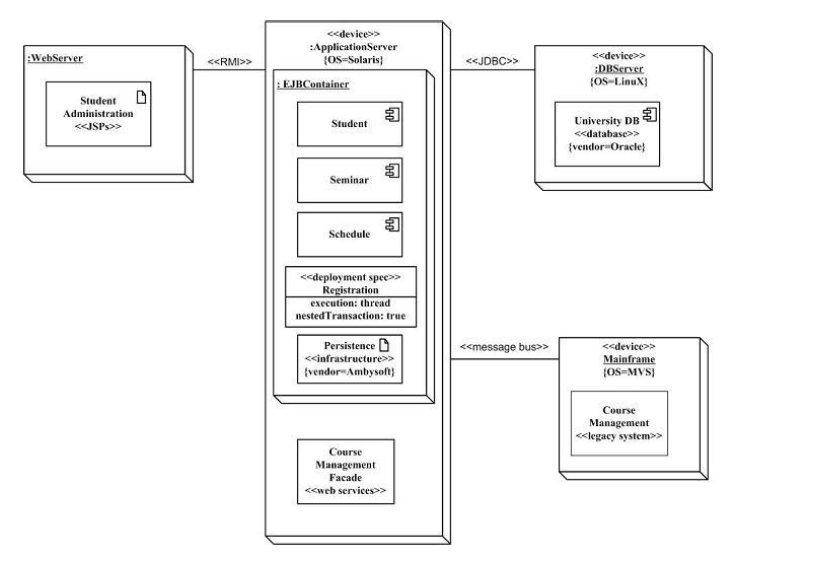
\includegraphics[width=4in]{img/deployment}%
\end{center}

\subsection{Deploymentdiagram: concepten}

De volgende concepten zijn van belang bij het opmaken van een deployment diagram :

\subsubsection{node}

\textbf{Node} is een algemene term, een aanduiding voor elk type computerelement (computers, monitors, printers, enz. enz.).

Men kan een onderscheid maken tussen twee types noden :

\begin{enumerate}
    \item een processor:
    
    een node die een component kan uitvoeren
    \item een device:
    
    een node die geen component kan uitvoeren
    
\end{enumerate}

$\Rightarrow$ een device is op de een of andere manier een interface naar de buitenwereld

%afbeelding nog plaatsen

\begin{center}
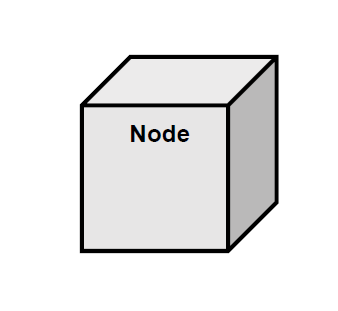
\includegraphics[width=2in]{img/node}%
\end{center}

Een node wordt voorgesteld als een \textbf{kubus}, waarin men de naam van de node kan opnemen.
